\chapter{Pixels detectors for the new ATLAS Inner Tracker}
\label{chap:ITk}

In this Chapter the new ATLAS Inner Tracker (ITk) of the ATLAS detector will be discussed. It is intended to be ready 
for  the data taking in 2026, in time for the beginning of the High Luminosity phase of the LHC (HL-LHC). 
The plans for the upgrades of the LHC are presented in Section~\ref{sec:HL-LHC}, along with the 
physics case and the list of ATLAS sub detector upgrades for the Phase-II; 
Section~\ref{sec:NewTracker} will cover the performance and specifications for the new ATLAS ITk. 
After describing the R\&D efforts for ITk pixels detectors in general (Section~\ref{sec:ITkPixels}), 
in Section~\ref{sec:radhardpixels} results for radiation hard pixel sensors will be presented. 
The concept of slim edge, already applied to IBL pixel sensors (Section~\ref{sec:IBLoverview}) will be 
pushed to its limits for the ITk pixels sensors; this topic will be discussed in details in 
Section~\ref{sec:edgeless}, together with results from beam tests. 
Finally conclusions and perspectives will be drawn in Section~\ref{sec:itksummary}.



\section{High Luminosity LHC and the Phase-II of the LHC experiments}
\label{sec:HL-LHC}

The timeline of the CERN LHC is presented in Figure~\ref{fig:HL-LHC-plan-2016-01}, together 
with the future plans. The High Luminosity LHC (HL-LHC)~\cite{HL_LHC} is a project, recently 
approved~\cite{HL-LHCApproval},  to upgrade the existing LHC to a high luminosity machine, 
capable to deliver an instantaneous luminosity of $L=7.5\times10^{34}$/cm$^{2}$/s; as a 
reminder the design luminosity of LHC is of $L=1.0\times10^{34}$/cm$^{2}$/s.
\begin{figure}[!htpb]
\centering
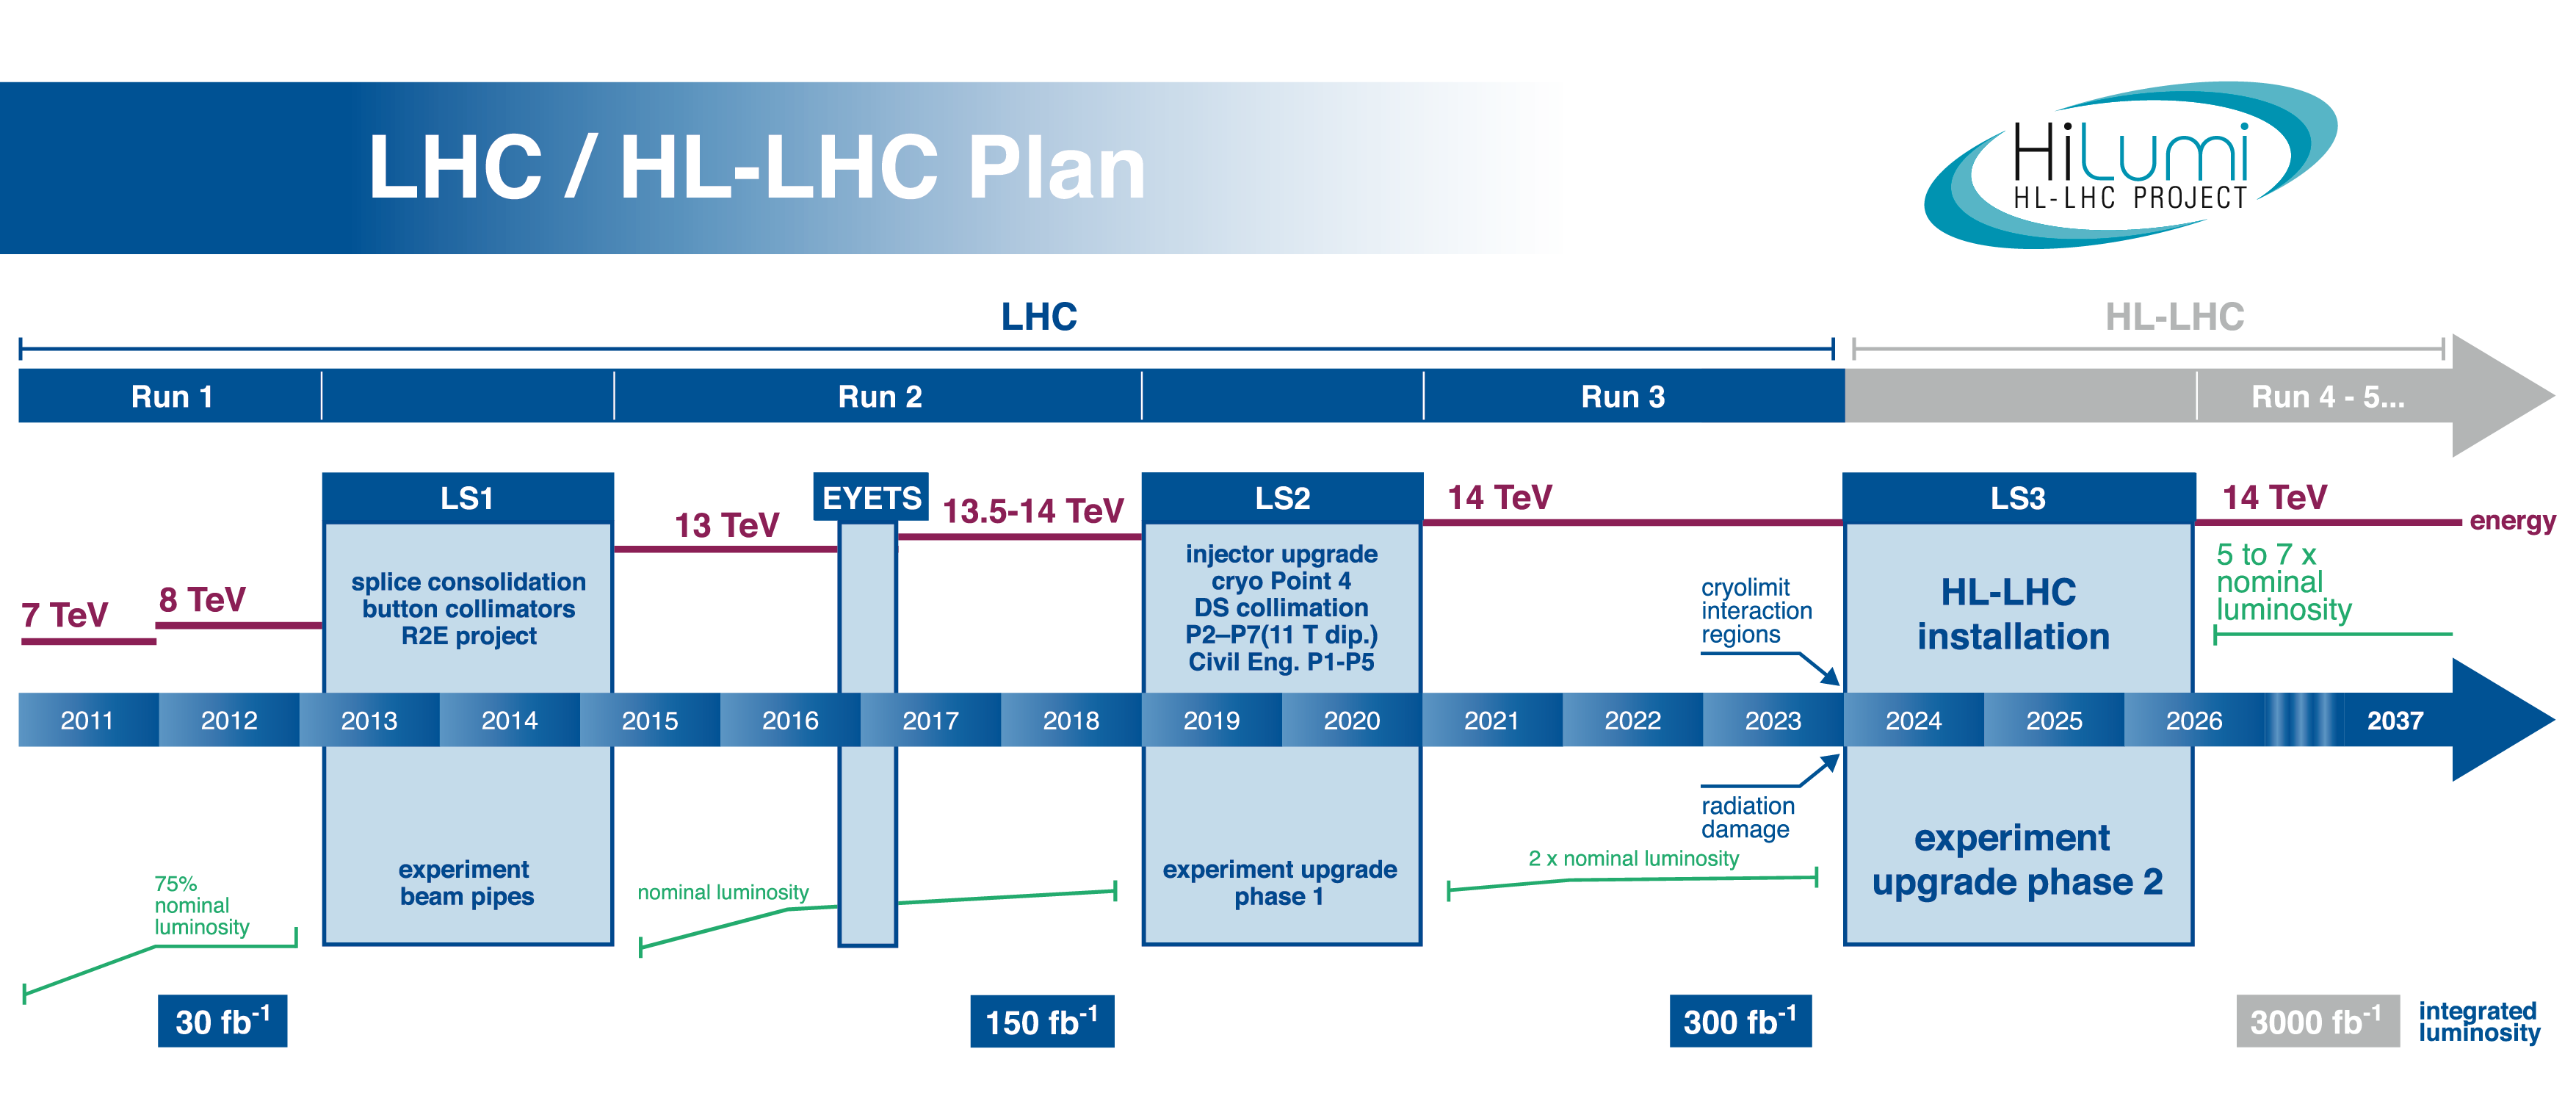
\includegraphics[width=1.0\textwidth]{HL-LHC-plan-2016-01.png}
\caption{\label{fig:HL-LHC-plan-2016-01}LHC/ HL-LHC Plan (last update 22.02.2016, after~\cite{HL_LHC})}
\end{figure}
After the HL-LHC upgrade completion the data taking  is expected to restart in 2026; the goal 
is to integrate a dataset of 3000~\invfb by 2037; there is an option to extend this program to arrive 
at 4000~\invfb.

As it can be seen in Figure~\ref{fig:HL-LHC-plan-2016-01} the upgrade plans don't include any increase 
of the center-of-mass energy $\sqrt{s}$. Thus, the main motivation for the HL-LHC project is 
reducing the error halving time. Indeed, taking data beyond 2023 at the same instantaneous luminosity of 
Run~3 would imply  to take data for more than 15 years to reduce the statistical error by a factor of 2.

The large dataset at the end of the so-called Phase 2 (or {\it} Phase-II) for the experiments should enable 
a  large program of precision measurements of the Higgs boson and New Physics (NP) discoveries. 
As an example of the potential of the HL-LHC dataset, the projected precision on coupling of the Higgs
 boson to $\mu$s is of about 7\% with  3000~\invfb; the Higgs 
trilinear self coupling parameter $\lambda_{HHH}$ can be probed at about 1 $\sigma$ significance 
in the range $-0.8<\lambda_{HHH}/\lambda_{SM}<7.7$ ($\lambda_{SM}$ is the SM predicted value) 
in the final state $HH\to\b\bbar\gamma\gamma$~\cite{ATL-PHYS-PUB-2014-016}. 
For what concerns NP potential discoveries, as an example, with the expected HL-LHC dataset the 
supersymmetric\footnote{Supersymmetry (SUSY) is a proposed type of spacetime symmetry where  each 
SM particle is associated with another particle, known as its superpartner, the spin of which differs by a 
half-integer; for an introduction to SUSY see~\cite{SusyPrimer}} top quark partner $\widetilde{t}$, 
the {\it stop}, discovery mass range extends up to 480~GeV, and the exclusion one to 700~GeV~\cite{ATL-PHYS-PUB-2016-022};
for the electroweak SUSY particles a factor of ten increase in luminosity translates into a 30-40\% increase in mass reach. Other than SUSY the physics program 
during the Phase-II of the LHC experiments include searches of   vector bosons resonances like 
$W',Z'$, 
extra dimensions and more~\cite{ATLASLoIPhaseII}.

The high luminosity foreseen for the Phase-II implies a much harsher environment than in Run~2 
for the ATLAS sub-detectors; indeed high luminosity means higher event rate, more pileup events 
and higher radiation doses and fluences. 
To cope with the severe data taking conditions expected at the HL-LHC it is planned to 
upgrade the  ATLAS detector~\cite{ATLASLoIPhaseII,ATLASITkScopingDocument}. Upgrades include:

\begin{itemize}
\item a longer latency trigger system, to cope with higher event rates,
\item new inner muon barrel trigger chambers, to assure redundancy and improve efficiency,
\item upgrading the tile calorimeter electronics, since the actual system will not survive the doses expected by the time of HL-LHC and
\item a complete new silicon only tracker, with coverage down to pseudorapidity $|\eta|=4$, the {\it Inner Tracker} (ITk)
\end{itemize} 

The constraints, requirements, layout and expected performance of the proposed ATLAS ITk will 
be discussed in the next Section.

\section{The Quest for a New ATLAS Inner Tracker}
\label{sec:NewTracker}

The new ATLAS  Inner Tracker will have to face unprecedented levels of radiation doses and fluences, 
pileup events and events rate. Table~\ref{tab:ITkConditions} summarises some of the most important figures.

\begin{table}[!htpb]
\centering
\caption{\label{tab:ITkConditions}Environment conditions for the inner detector at the LHC and HL-LHC}
\begin{tabular}{lcc}
\hline
\hline
Parameter & LHC & HL-LHC \\
\hline
instantaneous luminosity $L$	 [cm$^{-2}$s$^{-1}$] & $1.0\times10^{34}$ &  $7.5\times10^{34}$ \\
number of pileup events $\mu$ & 25 & 200\\
track rate density for the innermost pixel layer $\mathcal{N}$ [MHz~cm$^{-2}$] & 0.25 & 2 \\ 
fluence to the innermost pixel layer $\Phi$ [ 1 MeV $n_\text{eq}/\text{cm}^2$] & 5$\times10^{15}$ & 2$\times10^{16}$ \\
total ionising dose to the innermost pixel layer TID [MRad] & 160  & 1700 \\
\hline
\end{tabular}
\end{table}

Within this hostile environment the ITk will have to guarantee the same level of performance  or better 
of the ATLAS Inner Detector (ID).
The project is presented  in a series of documents, from the ``Letter of Intent for the Phase-II Upgrade of the ATLAS Experiment''~\cite{ATLASLoIPhaseII} to the ``ATLAS Phase-II Upgrade Scoping Document''~\cite{ATLASITkScopingDocument}. Technical Design Report (TDR) for strip detector of the 
ITk was recently published~\cite{ITkStripsTDR}; the ITk pixel detector TDR is due by the end of 2017.
This Section is built on those documents.




\subsection{Performance Requirements of the ITk}
In what follows a short list of performance requirements of the ITk.

\paragraph{Track Reconstruction Efficiency}
The required 
track reconstruction efficiency in the central part ($|\eta|<2.7$) has to be above 99\% for muons with 
$p_T$ above 3~GeV/c, above 85\% for pions (electrons) with 
$p_T$ above 1(5)~GeV/c.  Fake tracks rate has to be kept below 1\% to avoid degrading resolution of 
objects built using tracks, like tracks jets.

\paragraph{Track Resolution and Vertex Reconstrucion}
The resolution on transverse momentum will be better than 0.5\% up $|\eta|=1$ for muons of 100~GeV/c 
$p_T$ and will degrade moderately till $|\eta|=2$. For $|\eta|\ge2.7$ the solenoid field diminishes, 
particularly at low radius, leading to poorer $p_T$ resolution. 
Resolution on longitudinal (transverse) parameter $d_0(z_0)$ are required to be better than 100~$\mu$m 
in the very central region $|\eta|<0.5$ for tracks with $p_T$~=~1GeV/c and better than 8 (50)~$\mu$m  
in the limit of very large transverse momentum.  
 
 With 200 pile-up events, the mean separation of primary vertices is typically less than 1~mm.
 It is therefore not possible for all vertices in a triggered event to be reconstructed individually. However, it is important that high transverse momentum objects (muons, electrons and tracks in high transverse energy jets) coming from a common vertex can all be correctly associated to the same vertex with good efficiency.
  This requirement corresponds, in the case of $\t\tbar$ events, to the probability of the $\t\tbar$  vertex being among the reconstructed vertices having to be greater than 0.95. In addition, the probability that the 
$\t\tbar$  decay is associated to the correct reconstructed vertex should be greater than 0.90.
 
 
 Tracking-reconstruction efficiency and minimisation of multiple scattering effects requirements impose a 
 low material budget. For the ITk, generally it is required to be in total <1 $\X_0$ up to $|\eta|\le2.7$.
 In Figure~\ref{fig:ITk_X0}.
  The ITk material budget is around 30\% lower in the region $|\eta|\le4.0$, compared to the Run~2 detector.
\begin{figure}[!htpb]
\centering
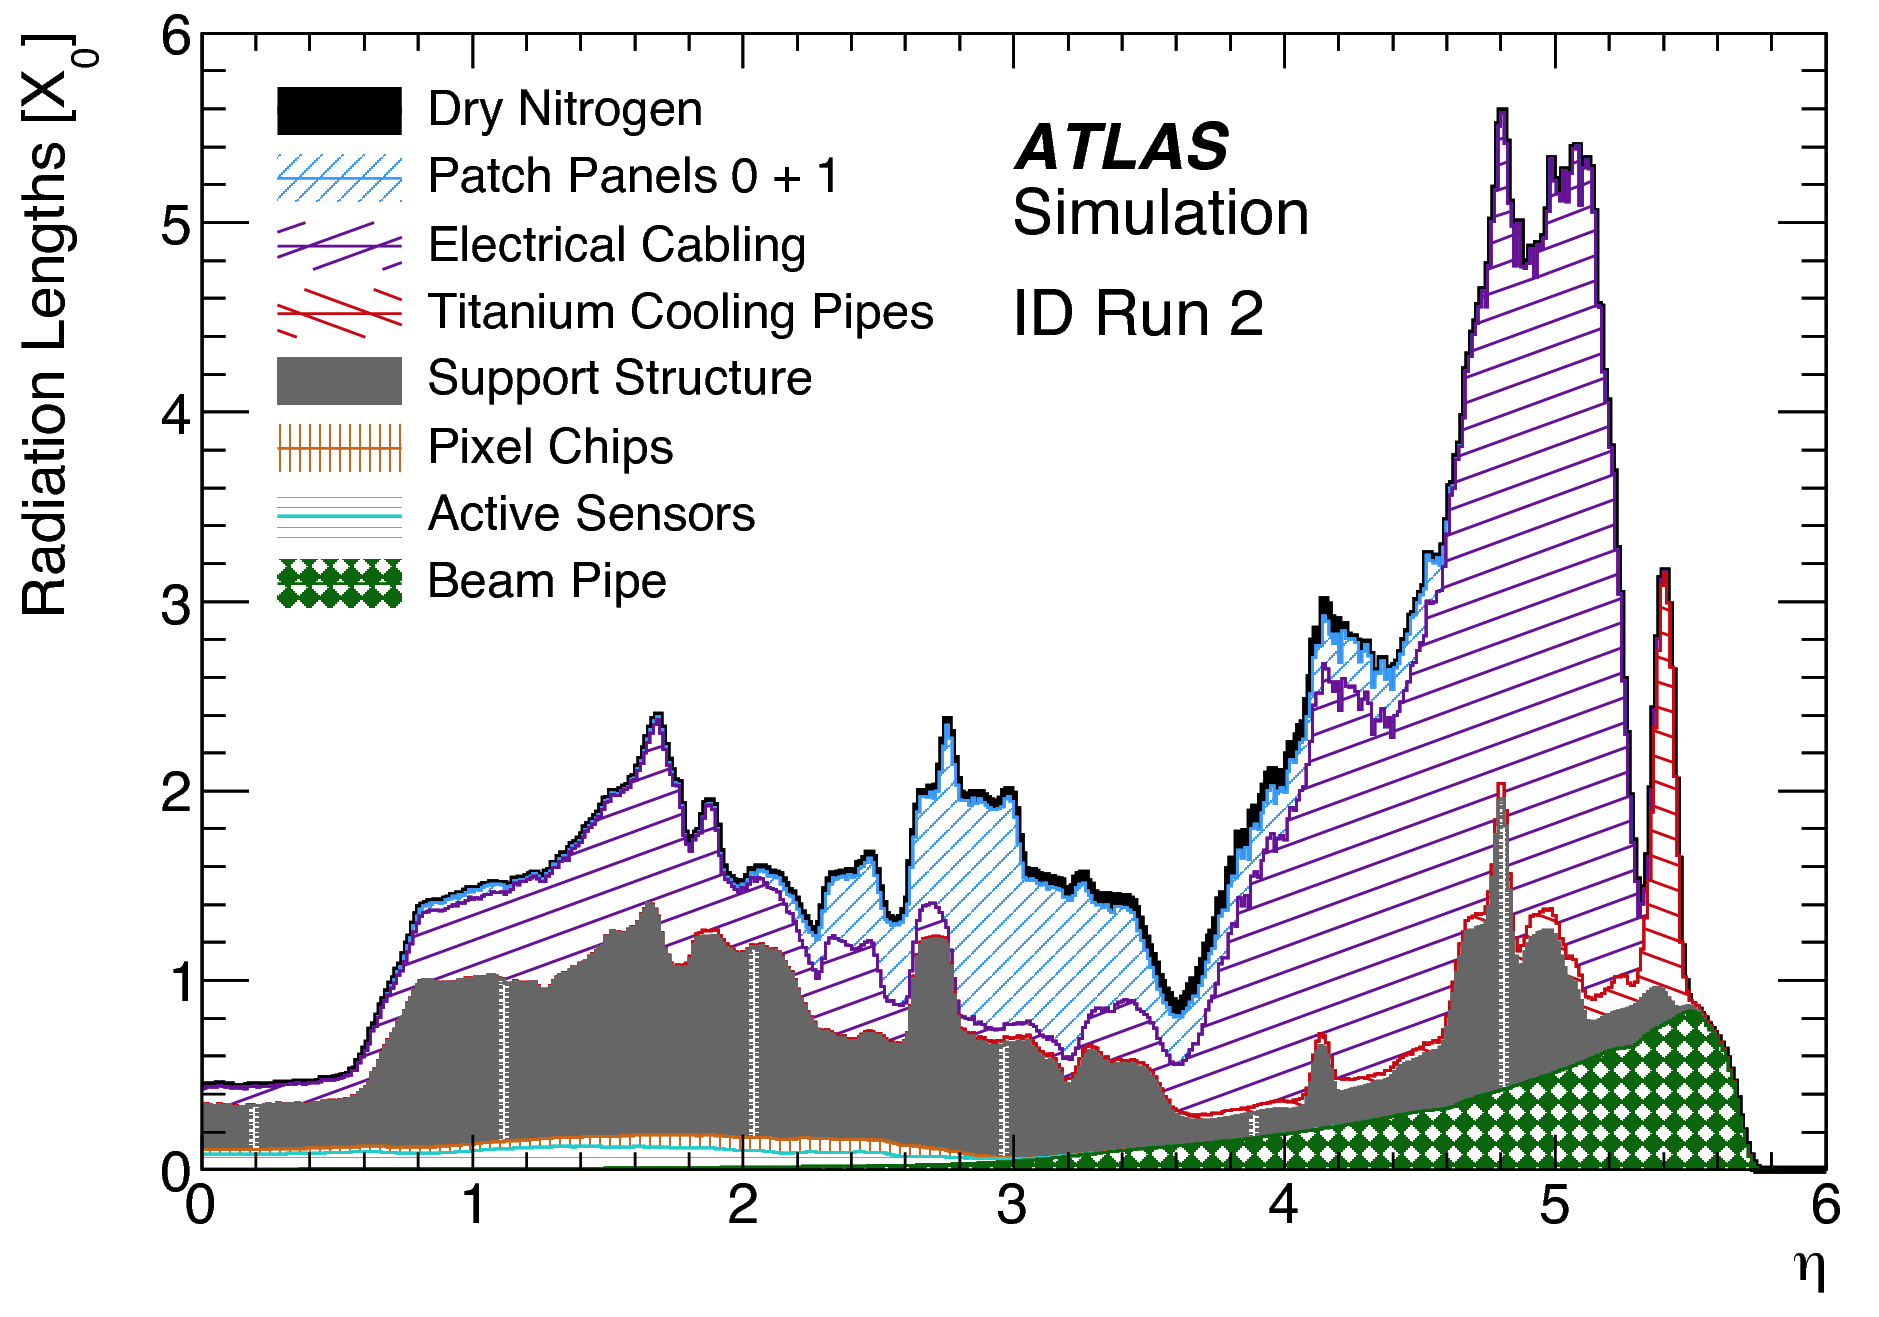
\includegraphics[width=0.49\textwidth]{ID_X0.png}
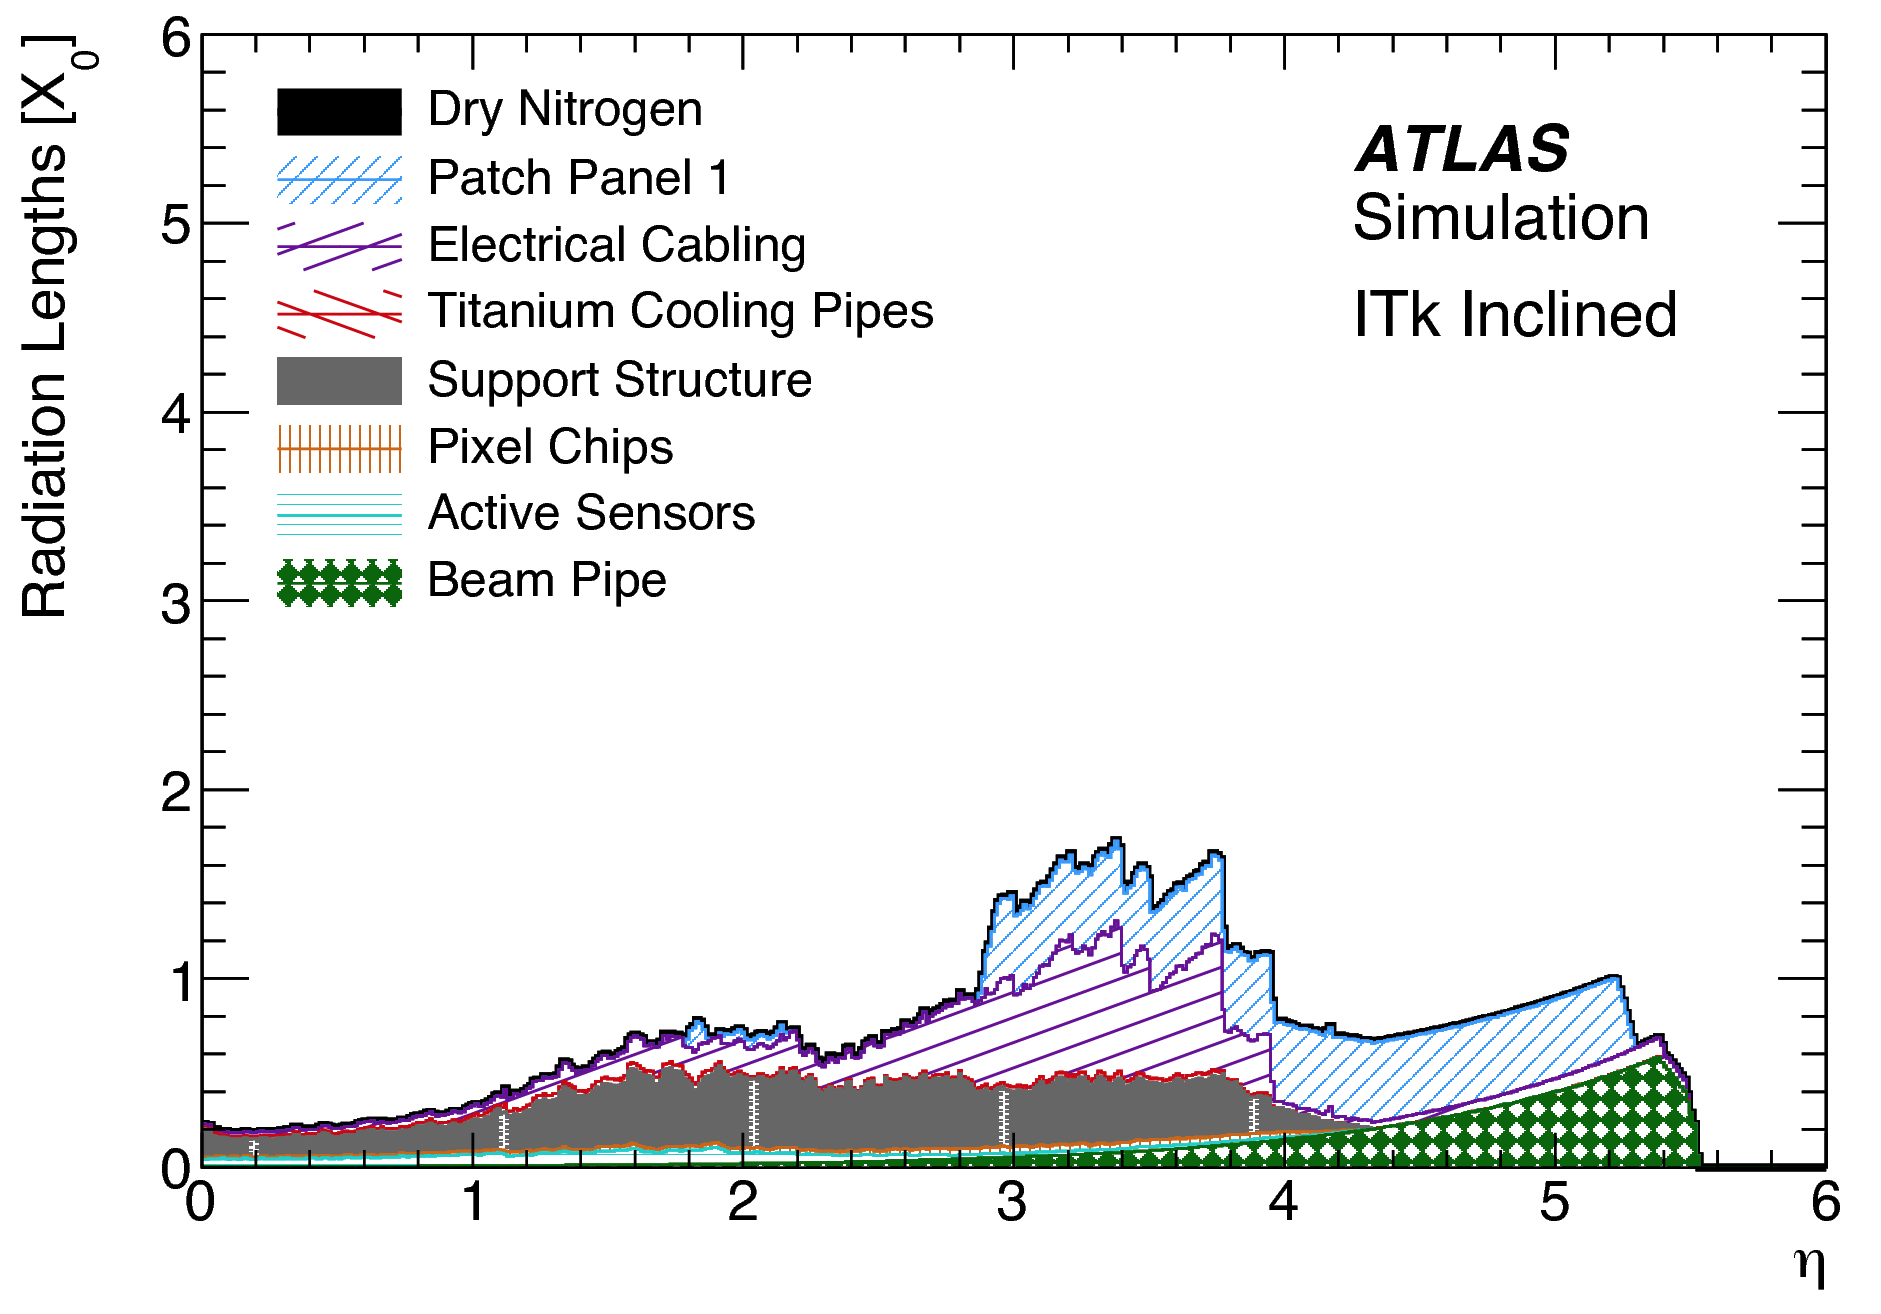
\includegraphics[width=0.49\textwidth]{ITk_X0.png}
\caption{\label{fig:ITk_X0}Material budget expressed as fraction of radiation lengths as a function of the 
pseudorapidity. (left) ATLAS ID (right) ATLAS ITk. (After~\cite{ITkStripsTDR})}
\end{figure}
  
\subsection{ITk detector layout}

The ITk will be an all silicon tracker; the main reason for abandoning the TRT is the projected occupancy 
in its straw tubes, which is about 100\% at $L=5.0\times10^{34}$cm$^{-2}$s$^{-1}$. 
The ITk will consist of an inner detector made of pixel modules and an outer one made of strips. 
In the central region of the ITk Detector, sensors are arranged in cylinders around the beam axis, with (starting from inside) five pixel layers followed by two short-strip layers of paired stereo modules then two long-strip layers of paired stereo modules. The forward regions will be covered by six strip disks and a number of pixel rings leading to one or more hits depending on the ring layer and $\eta$ position. 
The ITk layout is presented in Figure~\ref{fig:ITk_Layout}. The new tracker will cover a pseudorapidity range down to $|\eta|=4$. 

\begin{figure}[!htpb]
\centering
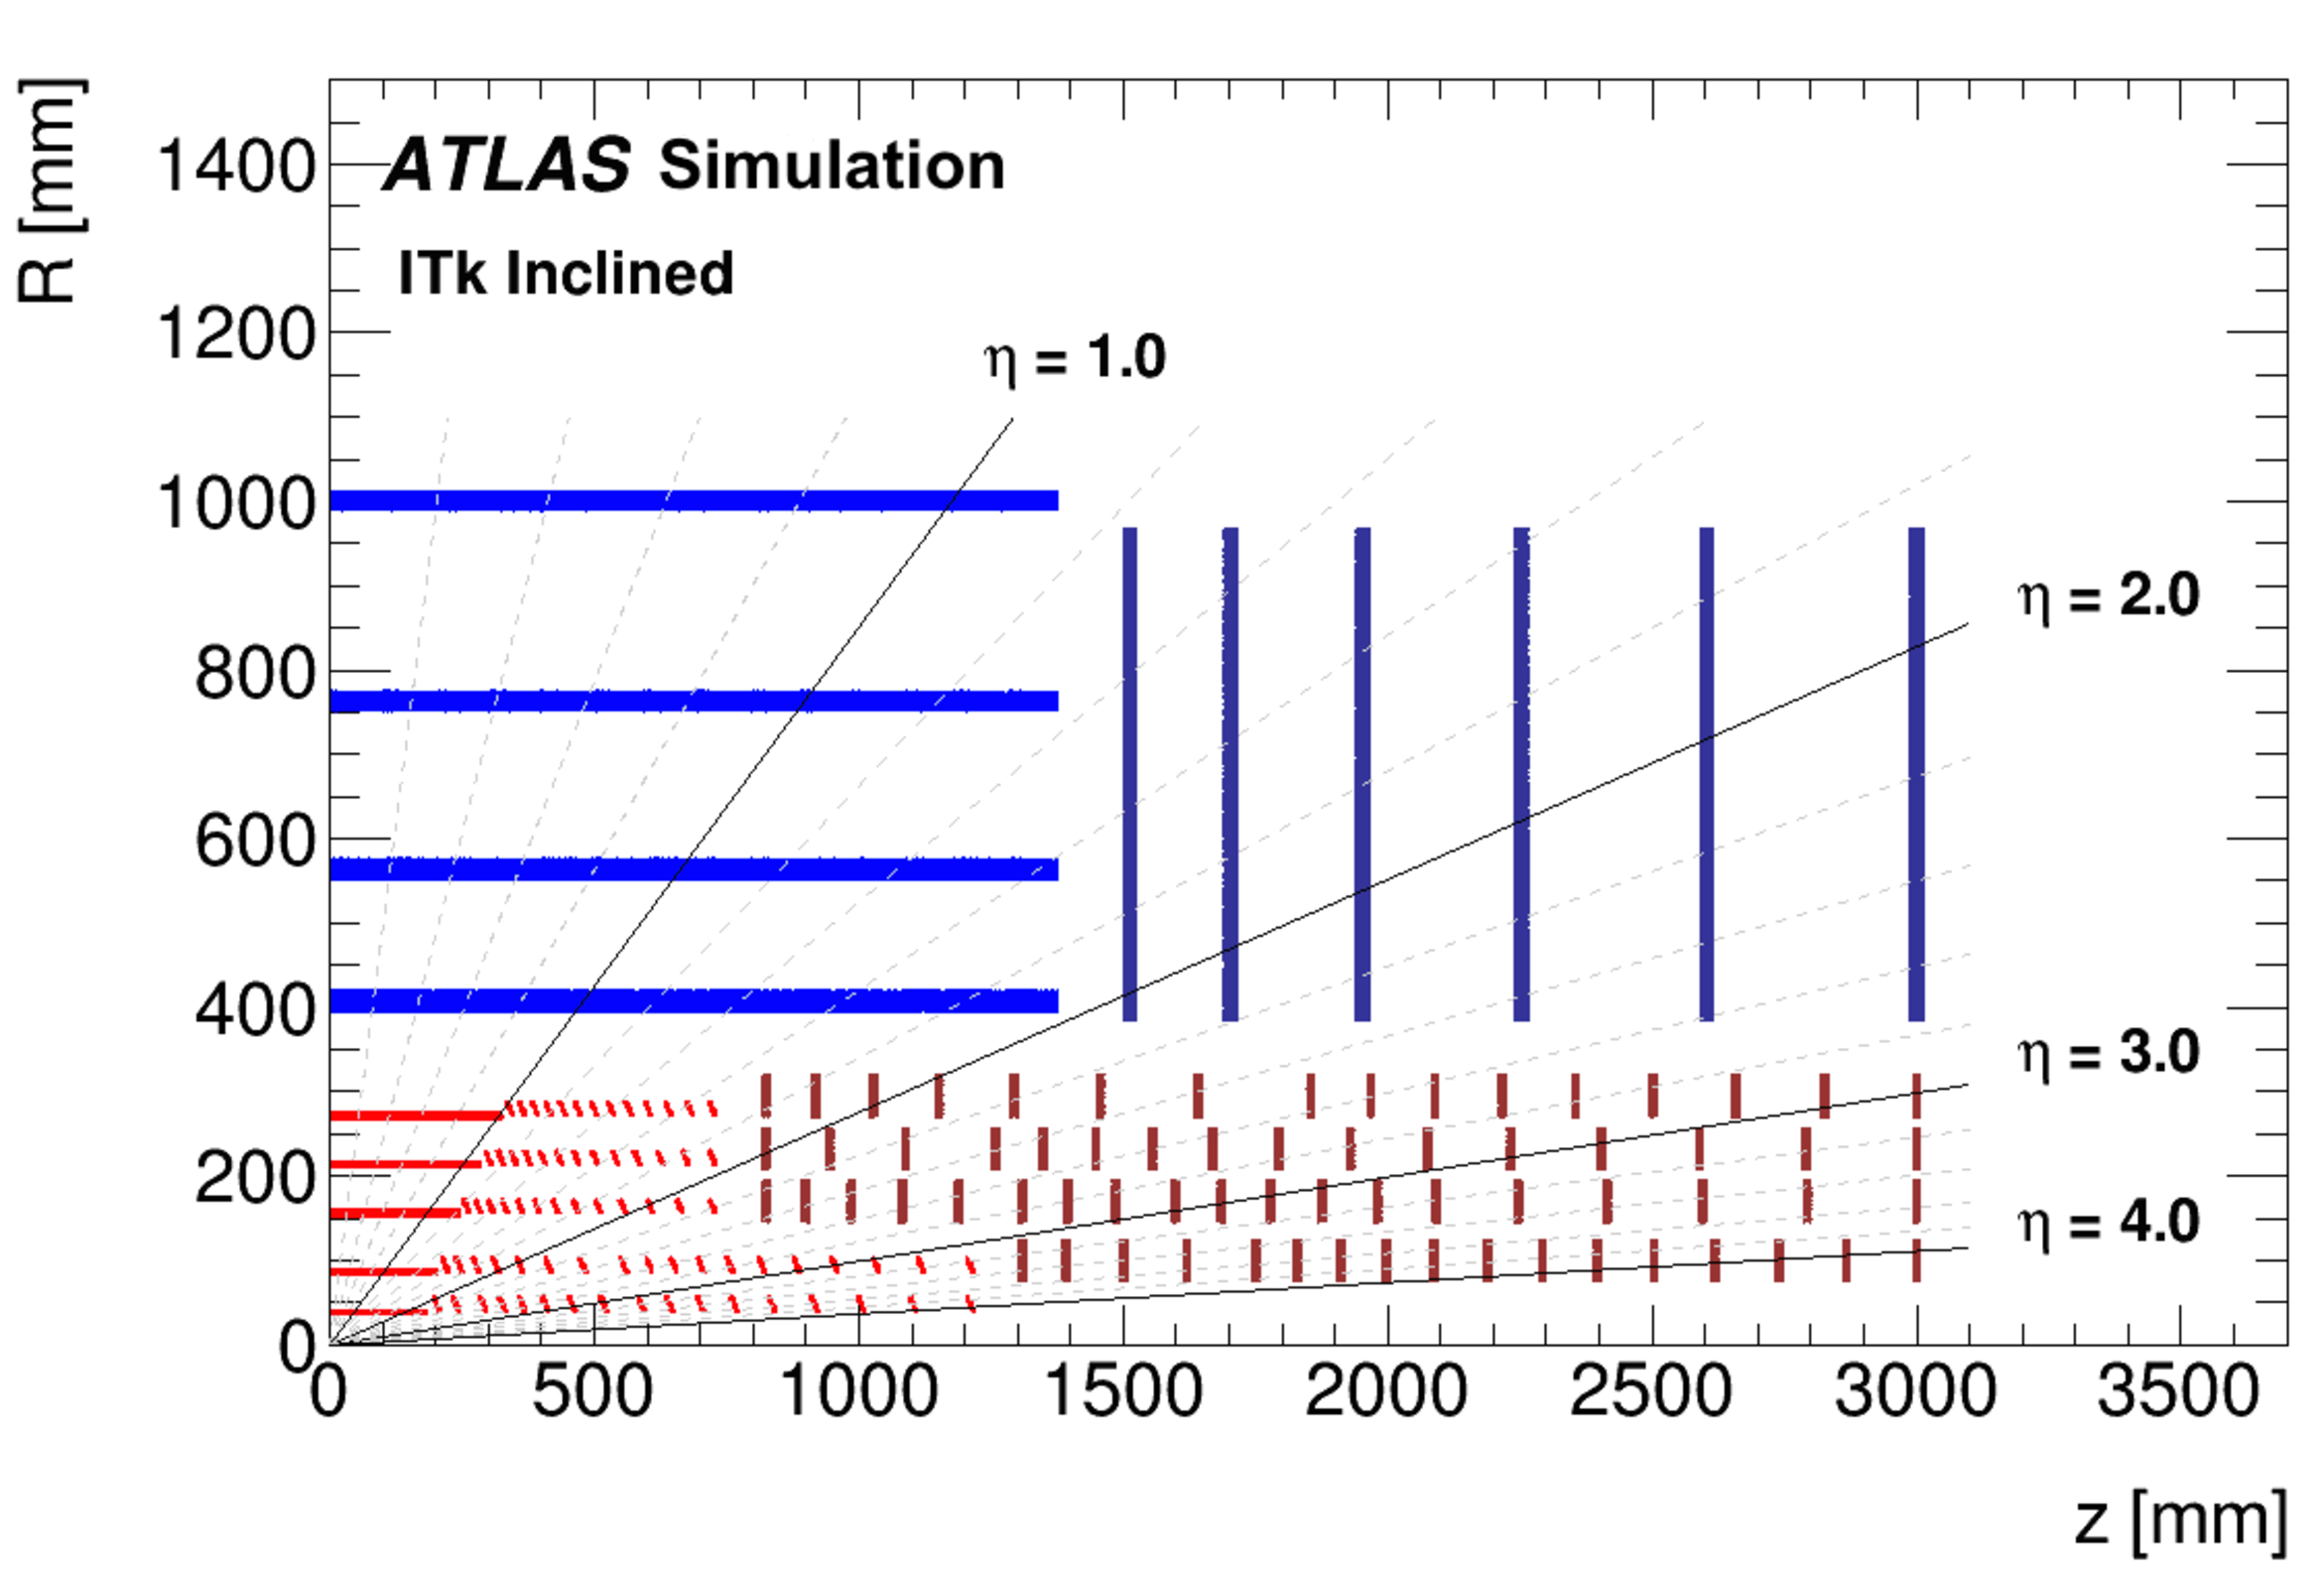
\includegraphics[width=0.65\textwidth]{ITk_Layout.pdf}
\caption{\label{fig:ITk_Layout}Schematic layout of the ITk for the HL-LHC phase of ATLAS. Here only one quadrant and only active detector elements are shown. The horizontal axis is the axis along the beam line with zero being the interaction point. The vertical axis is the radius measured from the interaction point. The outer radius is set by the bore of the solenoid. (After~\cite{ITkStripsTDR})}
\end{figure}

The peculiarity of the chosen ITk baseline layout, the so called ``Inclined'' layout, is the presence of 
inclined sensors in the forward part of the barrel layers; the inlined sensor hangs from  long 
barrel staves.
   This allows the material transversed by particles at 
large  $\eta$ to be minimised and at the same time requires less silicon surface to cover the full  $\eta$  
range. In addition, these inclined sensors provide two or more hits in the first layer, providing redundancy for the local track finding close to the interaction point even at large pseudorapidity.
One possible  support design of the Inclined layout is called ALPINE; a detail of the ALPINE stave 
prototype is shown in Figure~\ref{fig:ALPINE}.
\begin{figure}[!htpb]
\centering
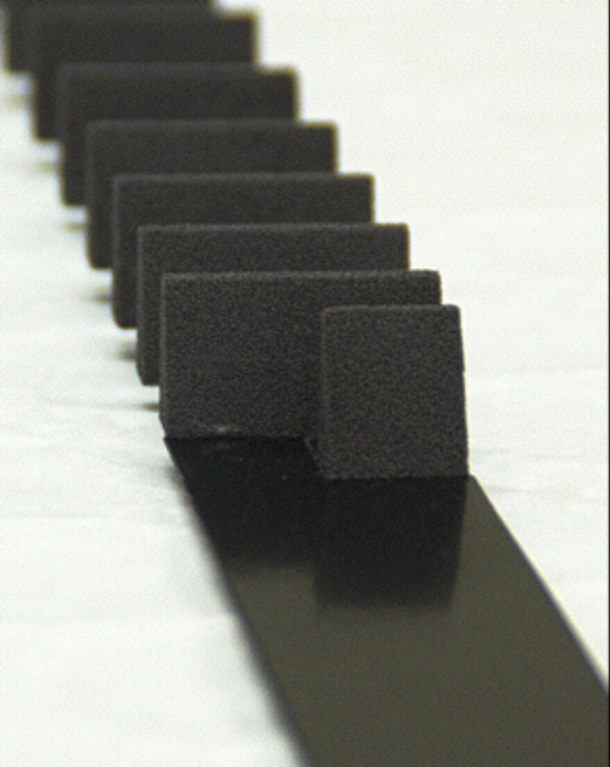
\includegraphics[height=0.25\textheight]{ALPINE.pdf}
\caption{\label{fig:ALPINE}ALPINE design for the inclined layout (After~\cite{ITkStripsTDR})}
\end{figure}
The sensor modules are located on the stave face closer to the interaction point so that incoming particles 
are detected by a pixel sensor before crossing the inactive material (local support structure, cooling tubes 
and electrical services).

\section{Pixels Detectors for ITK}
\label{sec:ITkPixels}

The innermost pixel barrel layer, Layer 0, of the ITk will be at about 40~mm; the Layer 1 at 85~mm. 
Layer 2, 3 and 4 will be placed respectively at 155, 213 and 271~mm from the beam axis. 
The expected fluences for the ITk are reported in Figure~\ref{fig:ITk_Fluence}.

\begin{figure}[!htpb]
\centering
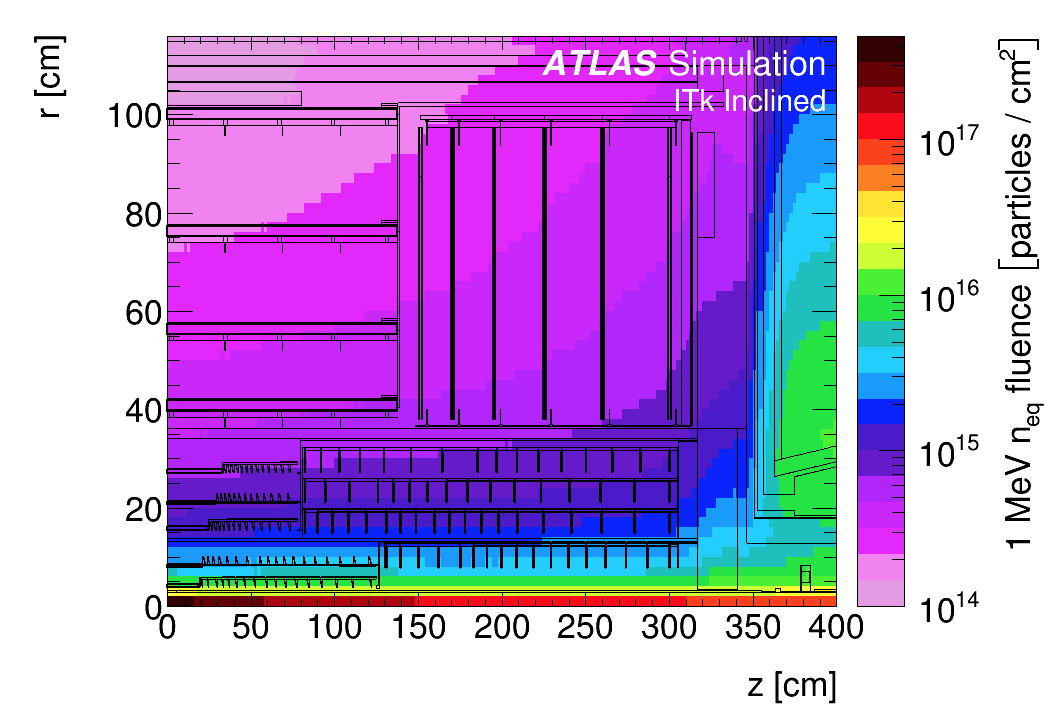
\includegraphics[width=0.65\textwidth]{ITk_Fluence.png}
\caption{\label{fig:ITk_Fluence} The 1 MeV neutron equivalent fluence  for the ITk layout 
(After~\cite{ITkStripsTDR})}
\end{figure}

The maximum fluence predicted for the Layer 0 at the end of the Phase-II program is about 1.5-2$\times10^{16}$~n$_{\rm eq}$/cm$^2$; for the pixel end-cap the largest fluence will be  of about 
5$\times10^{15}$~n$_{\rm eq}$/cm$^2$, similar to what it is expected for the Layer 1 of the barrel section.

Pixels will have a smaller pitch than today ATLAS pixel and IBL detectors; this is mandatory to keep  the 
occupancy below 1\%, in order to assure a good two particle separation and limit dead time. 
The proposed ITk layouts are designed to meet this requirement, thus the pixel pitches 
are dictated by this constraint. 
Moreover physics and performance simulations indicated that   50~$\mu$m~$\times$~50~$\mu$m pitch 
pixels, or 25~$\mu$m~$\times$~100~$\mu$m are suited (the smaller pitch is to achieve better 
momentum resolution).
Small pixel cells imply also less leakage current fed into and small capacitance coupled to the front end 
electronics, hence less noise. 


The basic  unit of the ITk pixel detector is a module. The baseline module concept for the ITk pixel detector is the well proven hybrid pixel detector in which modules are composed of a sensor and the read-out chip (ROIC) bump bonded to each other on a pixel level. In addition other concepts are also investigated such as monolithic CMOS pixel detectors especially for the outer layers.





The choice of sensors depends mainly on the requirement that the detector has to withstand the integration of an expected dataset  of 3000\invfb.  This is particularly challenging for the innermost layer, which after the high-luminosity running is exposed, as it was said above, to an estimated fluence $\Phi$ of 1.5-2$\times10^{16}$~n$_{\rm eq}$/cm$^2$ for the innermost pixel layer. 

There will be two main types of modules: dual-modules (two chips bump bonded to a sensor, around 
4~$\times$~2~cm$^2$) for the the innermost layer to accommodate the limited space, quad- modules (four 
chips bump bonded to a sensor, around 4 $\times$~4~cm$^2$ for the outer layers and in the rings. 
The read-out chip is presently under development within the RD53 collaboration~\cite{RD53}, 
which will produce an RD53 prototype chip. Following this chip an ATLAS ITk pixel chip will be developed 
using the basic blocks designed by RD53 while integrating additional functionality to meet ATLAS 
specifications.

At this stage three possible sensor types are considered for the pixels modules:

\begin{itemize}
\item planar sensors, for an hybrid detector
\item 3D sensors, again for an hybrid detector,
\item monolithic CMOS sensors
\end{itemize}

\paragraph{3D sensors}
3D silicon detectors are candidates to be used for the inner most layer(s) of the barrel pixel system and 
some of the inner end-cap rings due to their excellent radiation hardness at low operational voltages and 
moderate temperatures with low power dissipation compared to planar sensors.
The 3D sensors will be produced on either 4" or 6" high resistivity $p-$type wafers. 
The total thickness of the sensors will be 200~$\mu$m, and and the active thickness\footnote{sensors can be realised in thin high resistivity wafers bonded to thick low resistivity ones; at the end of the fabrication process the latter can be lapped, completely or not. This approach is used to realise thin planar sensors too} will be between 
150 and 200~$\mu$m, with 150~$\mu$m being the baseline. 
The 3D sensors shall be produced by etching the $p-$ and $n-$columns from the same side (single side process). At the moment the pixel geometry will have a single readout column in the centre of the pixel (1E), surrounded by four ohmic columns. Figure~\ref{fig:3D_design} shows the proposed design of the pixel 
cell for the ITk 3D pixel modules. 

\begin{figure}[!htpb]
\centering
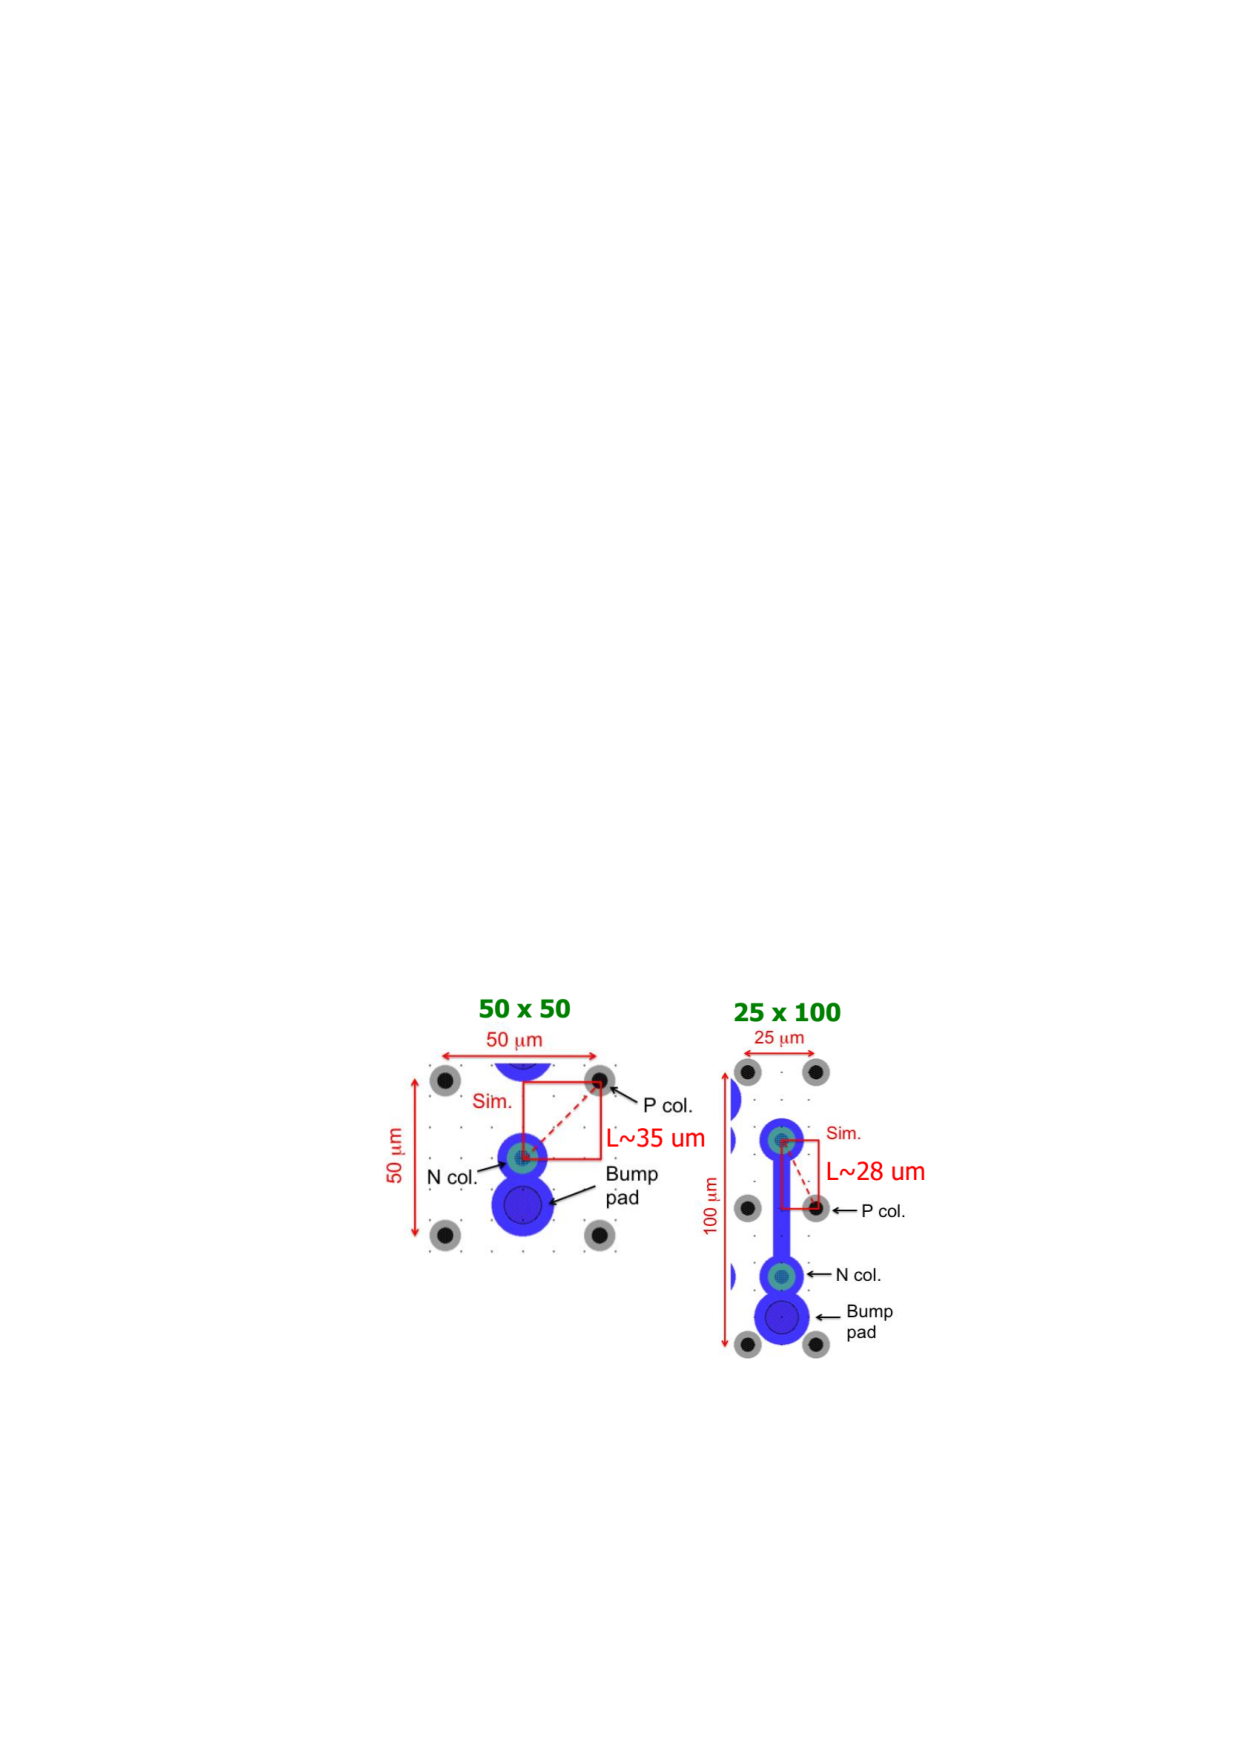
\includegraphics[width=0.55\textwidth]{3D_design.pdf}
\caption{\label{fig:3D_design} Design of 3D pixel cells with 50~$\mu$m~$\times$~50~$\mu$m  and 25~$\mu$m~$\times$~100~$\mu$m pitch pixels. (After~\cite{ITkStripsTDR})}
\end{figure}

The column diameter will be $\le$~8~$\mu$m, while the depth of the junction (ohmic) columns will be 
slightly shorter (longer) than the nominal  150~$\mu$m active thickness. Thus ohmic columns will 
be in contact with the sensor backside, while junction columns termination will be away from it, to 
avoid too early junction break down.

IBL-generation 3D pixel detectors coupled to FE-I4 pixel electronics have been found to have hit efficiencies 
in test beam measurements larger than 97\% at 170 V after irradiation to $\Phi$ of 
1.0$\times10^{16}$~n$_{\rm eq}$/cm$^2$ for normally incident minimum ionizing particles with a power 
dissipation of 15 mW/cm$^2$ at a temperature of -25$^{\circ}$~C~\cite{1748-0221-11-11-C11024}.

\paragraph{Planar sensors}
In this Paragraph only a short description of the planar sensors specification and performance 
for the ITk will be given as they will be discussed more in depth in the next two Sections. 
A new generation of planar pixel sensors are under development for the ATLAS ITk pixel system. The main 
differences with respect to the planar sensors implemented in the present detector are the different 
electrode arrangement ($n-in-p$ versus the traditional $n-in-n$) and the reduced thickness in the range of 
100-150~$\mu$m with respect to the 200~$\mu$m for the sensors used in IBL and 250~$\mu$m 
in the three outer ATLAS pixel layers. 

The $n-in-p$ technology allows for cost reduction given the single side processing and the reduced 
complexity in handling and testing. The guard ring structure is implemented on the front side, leaving the 
edges of the sensor at a potential close to the one of the backside. This arrangement potentially induces the 
risk of electrical sparks between the sensor periphery and the chip. Isolation techniques, like the deposition 
of a layer of Benzocyclobutene (BCB) on the sensor surface at wafer level or of parylene after module 
	assembly have been successfully employed to prevent this problem~\cite{Stefano,UNNO201372}.

\paragraph{Monolithic CMOS sensors}
Recent developments of CMOS pixel detectors, originally designed for charge collection in an epitaxial layer 
of 10-20~$\mu$m thickness, use new approaches to cope with the rate and radiation environment expected 
at the HL-LHC~\cite{PERIC2007876,1748-0221-11-02-C02045,HEMPEREK20158} 
based on the following enabling technology features:
HV add-ons that allow to use high depletion voltages; high resistivity wafers for large depletion depths; 
radiation hard processed with multiple nested wells to allow CMOS electronics em-bedded with sufficient 
shielding into the sensor substrate; and backside processing and
thinning for material minimisation and backside voltage application.

A typical CMOS sensor pixel cell with sensing substrate and a CMOS electronics layer
embedded in multiple cells is shown in Figure~\ref{fig:DMAPS}.

\begin{figure}[!htbp]
   \centering
   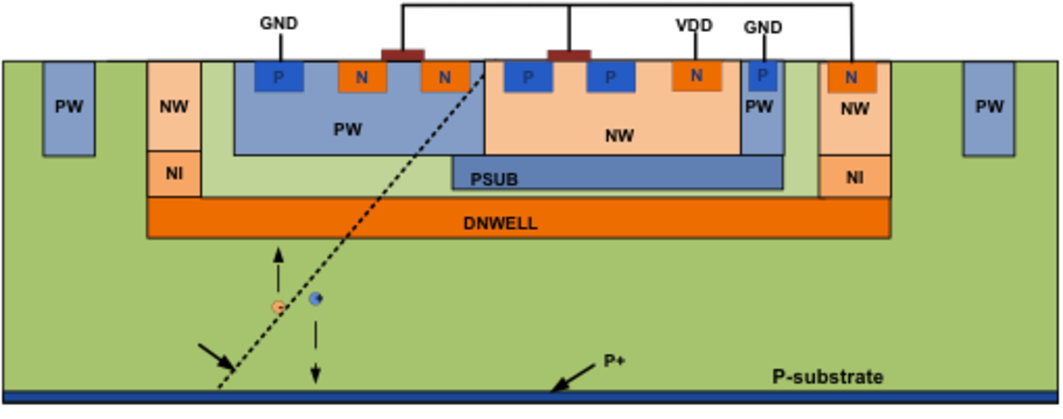
\includegraphics[width=0.65\textwidth]{DMAPS.pdf} 
   \caption{\label{fig:DMAPS}DMAPS schematic showing fully or partially depleted bulk, multiple nested wells for CMOS electronics and charge collection node. (After~\cite{ITkStripsTDR})}
   \end{figure}

Since 2014 a demonstrator programme to prove DMAPS that are suited for high rate and high radiation 
operation at LHC. For this a number of technologies have been explored and characterised 
(AMS 350 nm and 180 nm, Global Foundry 130 nm, ESPROS 150 nm, LFoundry 130nm, TowerJazz 
180nm, etc.); the designs have been characterised as stand-alone sensors as well as bonded to the FE-I4 
pixel chip (as a ?hybrid?) either via bump bonds or via glue bonding (capacitively coupled pixel detector, 
CCPD).

The results within the demonstrator programme can be summarised as follows:
\begin{itemize}
\item Technologies complying with the above list of enabling technology are principally suited to fabricate depleted monolithic sensors that can cope with the HL-LHC running condition, at least at distances larger than 20-25~cm away from the interaction point (outer layers).
\item DMAPS pixel sensors detect mips with integrated efficiencies above 98\% 
and with spatial resolutions similar to those as hybrid pixels 
\item DMAPS pixel sensors can stand radiation fluences of more than 1.0$\times10^{15}$~n$_{\rm eq}$/cm$^2$ when properly designed. This is demonstrated in Figure~\ref{fig:Eff_DMAPS} showing the 
collection width obtained after irradiation to a neutron fluence of 8.0$\times10^{15}$~n$_{\rm eq}$/cm$^2$ 
determined using
edge TCT measurements~\cite{1748-0221-12-02-P02021,5402213}.
\item  Test beam measurements have shown high rate capability as detectors bonded to the FE-I4.
\item Fully monolithic DMAPS pixel sensors have been designed incorporating read-out architectures suitable to cope with the expected rates at the HL-LHC (such as column- drain architectures and direct hit transfer architectures). Such designs have been sub- mitted for fabrication in 2016 and are currently being evaluated.
\end{itemize}

\begin{figure}[!htbp]
   \centering
   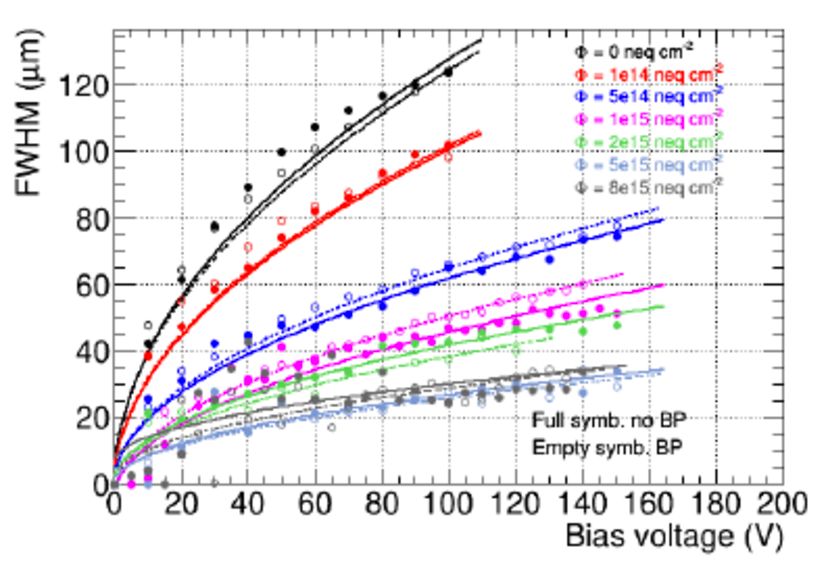
\includegraphics[width=0.6\textwidth]{Eff_DMAPS.pdf}
   \caption{\label{fig:Eff_DMAPS}FWHM of the charge collection profile measures using the edge TCT 
   technique  as a function of bias voltage after 
   different irradiation fluences up to 8.0$\times10^{15}$~n$_{\rm eq}$/cm$^2$ for un-thinned detector 
   (700~$\mu$m thick) without back plane (full symbols) and 300~$\mu$m
    sample with back plane
(empty symbols). 
(After~\cite{1748-0221-12-02-P02021})}
\end{figure}

\section{Radiation Hard Planar Pixel Sensors}
\label{sec:radhardpixels}

The ATLAS Upgrage Planar Pixel Sensor R\&D Project~\cite{PPS:proj}

\section{Edgeless Pixel Sensors}
\label{sec:edgeless}

The fractions of inactive regions are kept low by having larger pixels at the edge and in the regions between chips, and by minimising the edge region while still preventing voltage breakdown.

The 3D sensor technology inherently allows for slim edges of 15-150~$\mu$m~\cite{1748-0221-10-03-C03031}.
\section{Summary and Outlook}
\label{sec:itksummary}

